\documentclass[a4paper,12pt]{extarticle}
\usepackage[utf8x]{inputenc}
\usepackage[T1,T2A]{fontenc}
\usepackage[russian]{babel}
\usepackage{hyperref}
\usepackage{indentfirst}
\usepackage{listings}
\usepackage{color}
\usepackage{here}
\usepackage{array}
\usepackage{multirow}
\usepackage{graphicx}

\usepackage{caption}
\renewcommand{\lstlistingname}{Программа} % заголовок листингов кода

\bibliographystyle{ugost2008ls}

\usepackage{listings}
\lstset{ %
extendedchars=\true,
keepspaces=true,
language=C,						% choose the language of the code
basicstyle=\footnotesize,		% the size of the fonts that are used for the code
numbers=left,					% where to put the line-numbers
numberstyle=\footnotesize,		% the size of the fonts that are used for the line-numbers
stepnumber=1,					% the step between two line-numbers. If it is 1 each line will be numbered
numbersep=5pt,					% how far the line-numbers are from the code
backgroundcolor=\color{white},	% choose the background color. You must add \usepackage{color}
showspaces=false				% show spaces adding particular underscores
showstringspaces=false,			% underline spaces within strings
showtabs=false,					% show tabs within strings adding particular underscores
frame=single,           		% adds a frame around the code
tabsize=2,						% sets default tabsize to 2 spaces
captionpos=t,					% sets the caption-position to top
breaklines=true,				% sets automatic line breaking
breakatwhitespace=false,		% sets if automatic breaks should only happen at whitespace
escapeinside={\%*}{*)},			% if you want to add a comment within your code
postbreak=\raisebox{0ex}[0ex][0ex]{\ensuremath{\color{red}\hookrightarrow\space}},
texcl=true,
inputpath=listings,                     % директория с листингами
}

\usepackage[left=2cm,right=2cm,
top=2cm,bottom=2cm,bindingoffset=0cm]{geometry}

%% Нумерация картинок по секциям
\usepackage{chngcntr}
\counterwithin{figure}{section}
\counterwithin{table}{section}

%%Точки нумерации заголовков
\usepackage{titlesec}
\titlelabel{\thetitle.\quad}
\usepackage[dotinlabels]{titletoc}

%% Оформления подписи рисунка
\addto\captionsrussian{\renewcommand{\figurename}{Рисунок}}
\captionsetup[figure]{labelsep = period}

%% Подпись таблицы
\DeclareCaptionFormat{hfillstart}{\hfill#1#2#3\par}
\captionsetup[table]{format=hfillstart,labelsep=newline,justification=centering,skip=-10pt,textfont=bf}

%% Путь к каталогу с рисунками
\graphicspath{{fig/}}

%% Внесение titlepage в учёт счётчика страниц
\makeatletter
\renewenvironment{titlepage} {
 \thispagestyle{empty}
}
\makeatother

\usepackage{amsmath}

\begin{document}	% начало документа

% Титульная страница
\begin{titlepage}	% начало титульной страницы

	\begin{center}		% выравнивание по центру

		\large Санкт-Петербургский политехнический университет Петра Великого\\
		\large Институт компьютерных наук и технологий \\
		\large Кафедра компьютерных систем и программных технологий\\[6cm]
		% название института, затем отступ 6см
		
		\huge Название предмета\\[0.5cm] % название работы, затем отступ 0,5см
		\large Отчет по лабораторной работе №1\\[0.1cm]
		\large Тема работы\\[5cm]

	\end{center}


	\begin{flushright} % выравнивание по правому краю
		\begin{minipage}{0.25\textwidth} % врезка в половину ширины текста
			\begin{flushleft} % выровнять её содержимое по левому краю

				\large\textbf{Работу выполнил:}\\
				\large Петров В.Д.\\
				\large {Группа:} 43501/4\\
				
				\large \textbf{Преподаватель:}\\
				\large Ицыксон В.М.

			\end{flushleft}
		\end{minipage}
	\end{flushright}
	
	\vfill % заполнить всё доступное ниже пространство

	\begin{center}
	\large Санкт-Петербург\\
	\large \the\year % вывести дату
	\end{center} % закончить выравнивание по центру

\end{titlepage} % конец титульной страницы

\vfill % заполнить всё доступное ниже пространство


% Содержание
% Содержание
\renewcommand\contentsname{\centerline{Содержание}}
\tableofcontents
\newpage




\section{Цель работы}
Ознакомиться со способами выделения контуров при помощи операторов Робертса, Превитта и Собеля.


\section{Программа работы}
1. Выделить границы тремя способами на естественном изображении с ярковыраженными границами

2. Выделить границы тремя способами на искусственном изображении с ярковыраженными границами 

3. Сравнить результаты работы разных операторов и сделать выводы.


\section{Ход выполнения работы}

Операторы Робертса 

$\begin{pmatrix}
	1 & 0\\ 
	0 & -1
\end{pmatrix}$ 
$\begin{pmatrix}
	0 & 1\\ 
	-1 & 0
\end{pmatrix}$ 


Операторы Собеля 

$\begin{pmatrix}
	-1 & -2 & -1\\ 
	0 & 0 & 0 \\
	1 & 2 & 1
\end{pmatrix}$ 
$\begin{pmatrix}
	-1 & 0 & 1\\ 
	-2 & 0 & 2 \\
	-1 & 0 & 1
\end{pmatrix}$ 


Операторы Превитта 

$\begin{pmatrix}
	-1 & -1 & -1\\ 
	0 & 0 & 0 \\
	1 & 1 & 1
\end{pmatrix}$ 
$\begin{pmatrix}
	-1 & 0 & 1\\ 
	-1 & 0 & 1 \\
	-1 & 0 & 1
\end{pmatrix}$ 

Магнитуда считается как $\sqrt{x^2 + y^2}$



\subsection{Выделить границы тремя способами на естественном изображении с ярковыраженными границами}

\begin{figure}[H]
	\begin{center}
		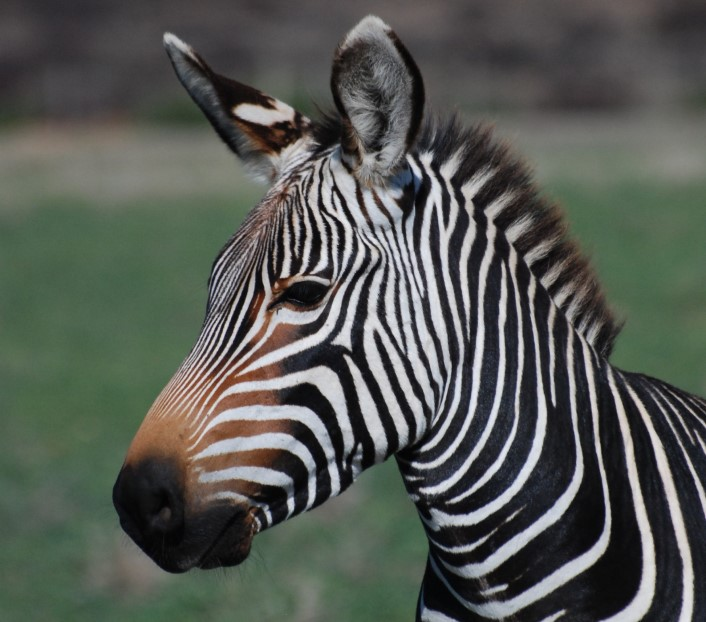
\includegraphics[scale=0.5]{zebra.jpg}
		\caption{Оригинальное изображение в цвете} 
		\label{pic:hist_orig} % название для ссылок внутри кода
	\end{center}
\end{figure}
\begin{figure}[H]
	\begin{center}
		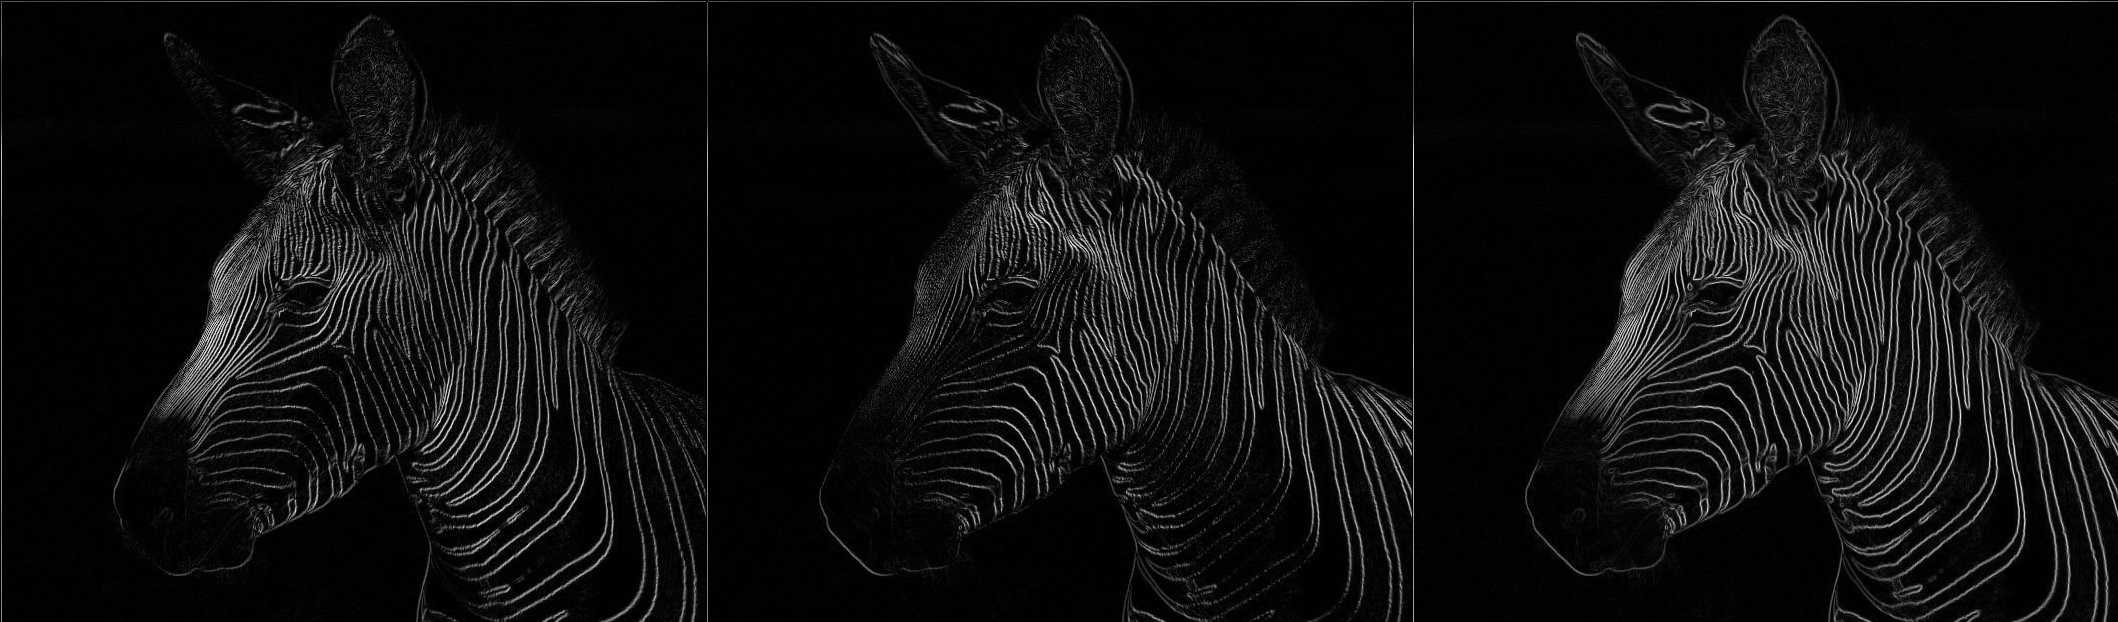
\includegraphics[scale=0.2]{robrts_all_2.jpg}
		\caption{Выделение границ при помощи операторов Робертса} 
		\label{pic:hist_orig} % название для ссылок внутри кода
	\end{center}
\end{figure}
\begin{figure}[H]
	\begin{center}
		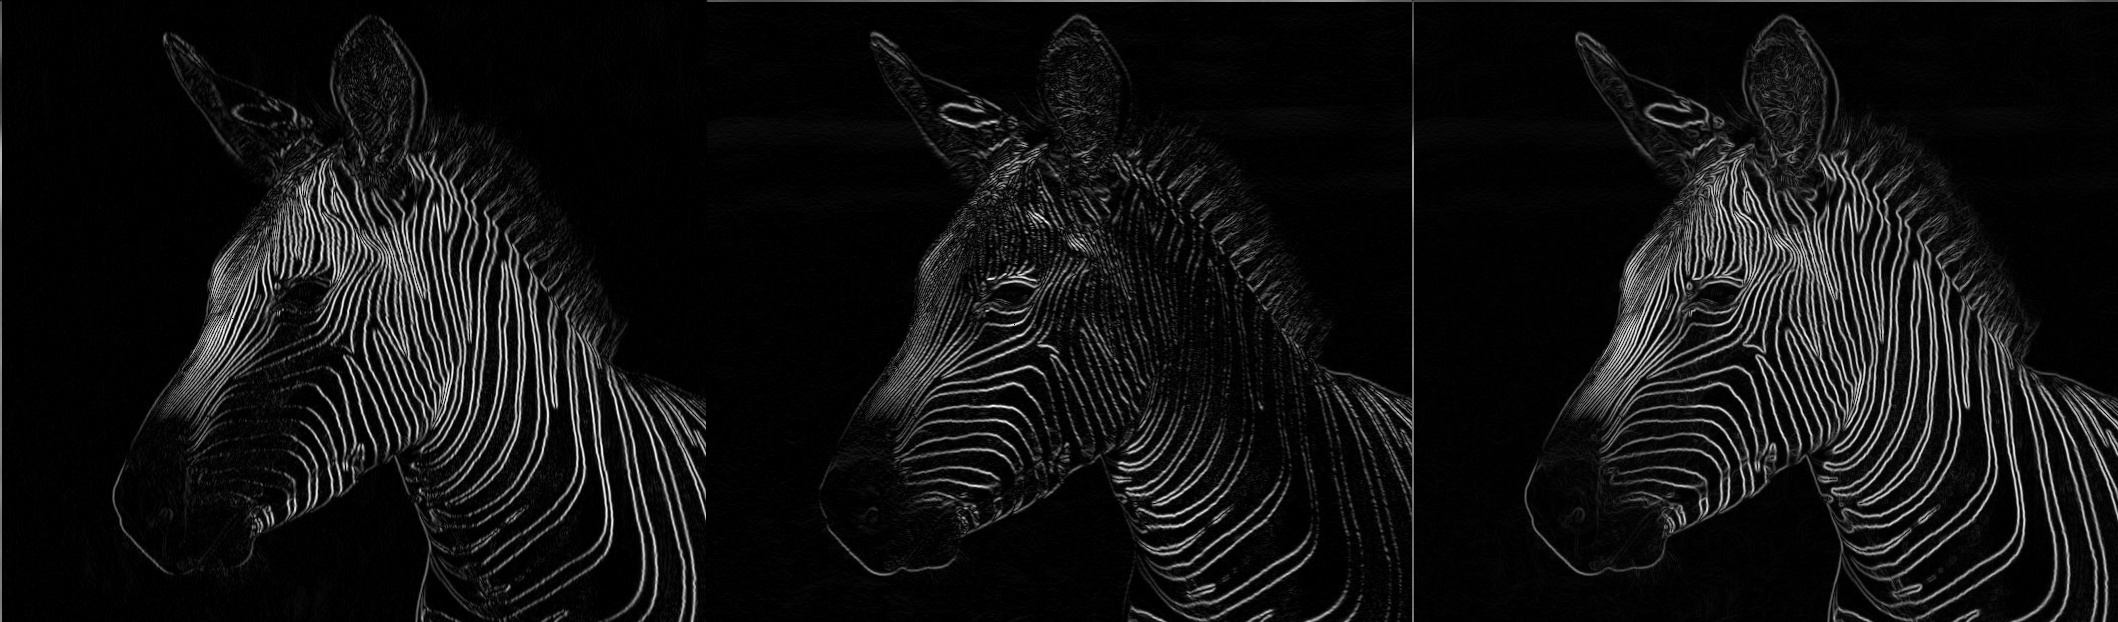
\includegraphics[scale=0.2]{Sobel_all_2.jpg}
		\caption{Выделение границ при помощи операторов Собеля} 
		\label{pic:hist_orig} % название для ссылок внутри кода
	\end{center}
\end{figure}
\begin{figure}[H]
	\begin{center}
		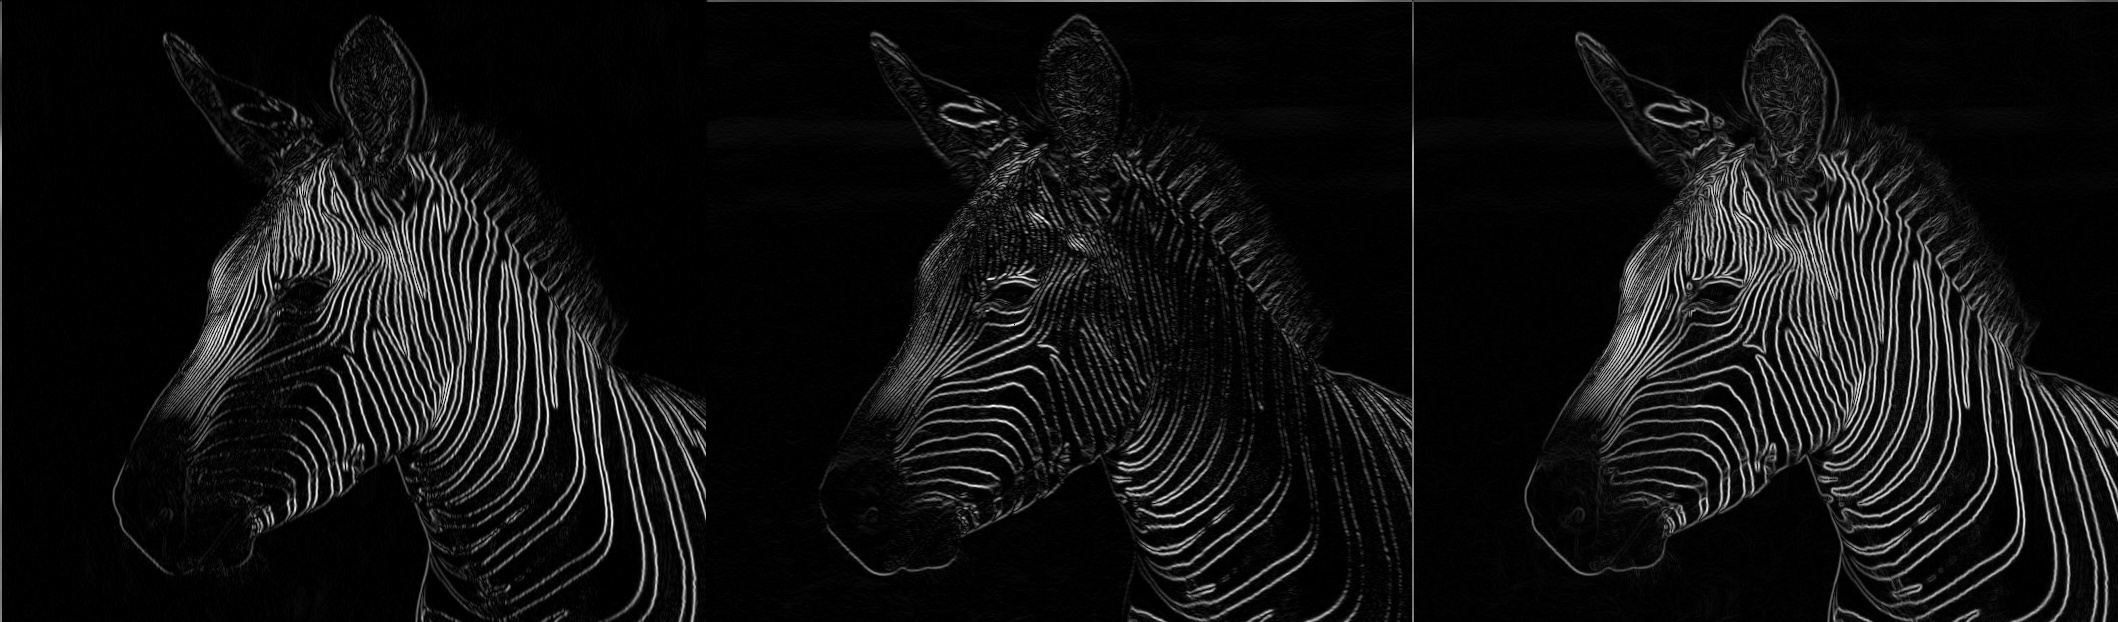
\includegraphics[scale=0.2]{prewit_all_2.jpg}
		\caption{Выделение границ при помощи операторов Превитта} 
		\label{pic:hist_orig} % название для ссылок внутри кода
	\end{center}
\end{figure}



\subsection{Выделить границы тремя способами на искусственном изображении с ярковыраженными границами}
\begin{figure}[H]
	\begin{center}
		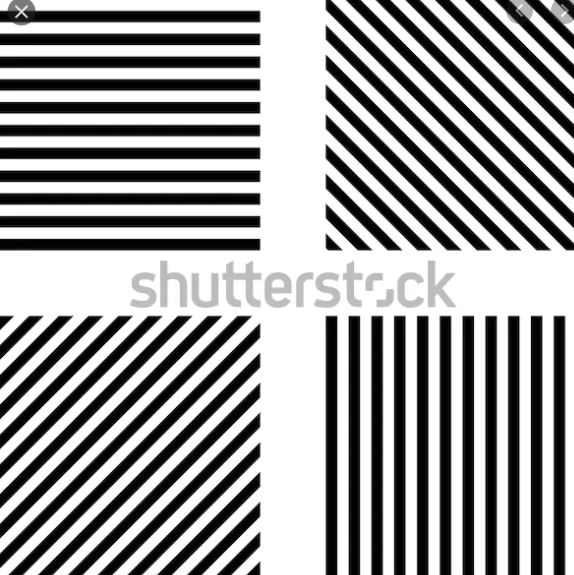
\includegraphics[scale=0.5]{lines.JPG}
		\caption{Оригинальное изображение} 
		\label{pic:hist_orig} % название для ссылок внутри кода
	\end{center}
\end{figure}
\begin{figure}[H]
	\begin{center}
		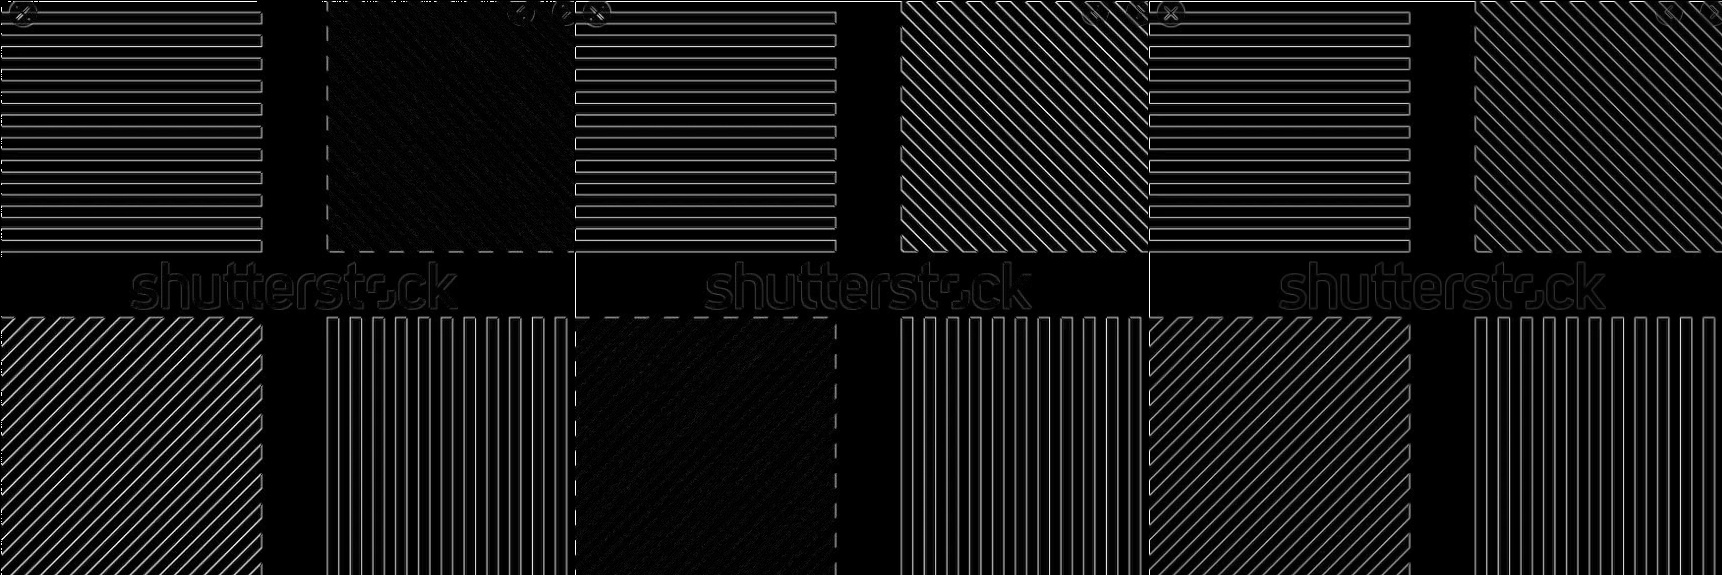
\includegraphics[scale=0.25]{robrts_all_1.jpg}
		\caption{Выделение границ при помощи операторов Робертса} 
		\label{pic:hist_orig} % название для ссылок внутри кода
	\end{center}
\end{figure}
\begin{figure}[H]
	\begin{center}
		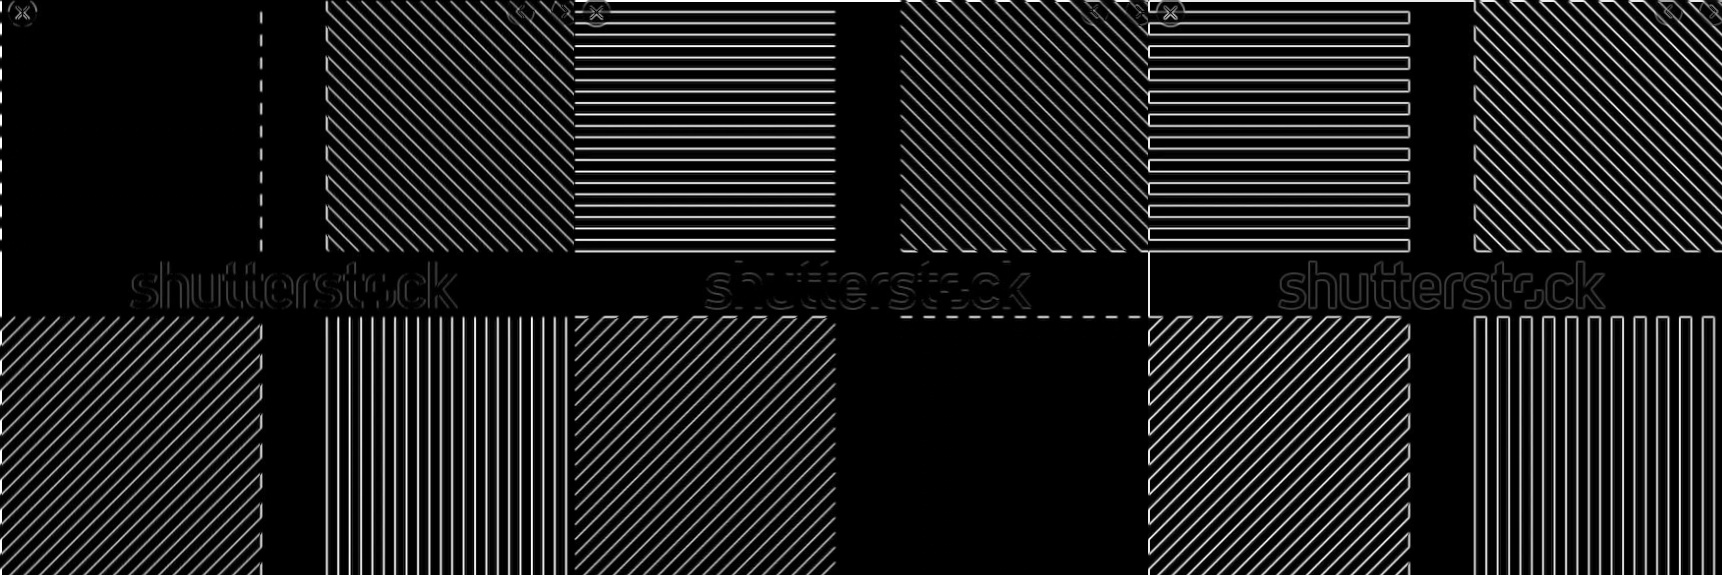
\includegraphics[scale=0.25]{Sobel_all_1.jpg}
		\caption{Выделение границ при помощи операторов Собеля} 
		\label{pic:hist_orig} % название для ссылок внутри кода
	\end{center}
\end{figure}
\begin{figure}[H]
	\begin{center}
		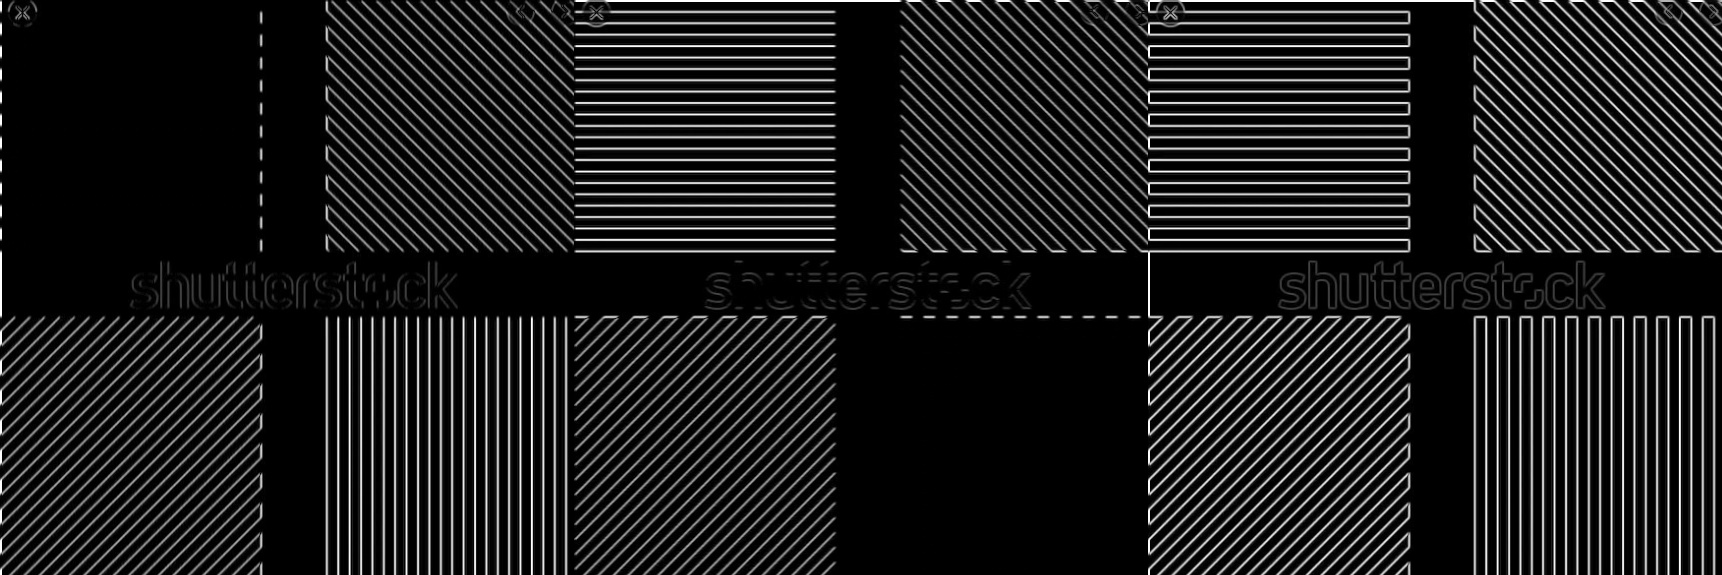
\includegraphics[scale=0.25]{prewit_all_1.jpg}
		\caption{Выделение границ при помощи операторов Превитта} 
		\label{pic:hist_orig} % название для ссылок внутри кода
	\end{center}
\end{figure}

\subsection{Сравнить результаты работы разных операторов и сделать выводы}

\begin{figure}[H]
	\begin{center}
		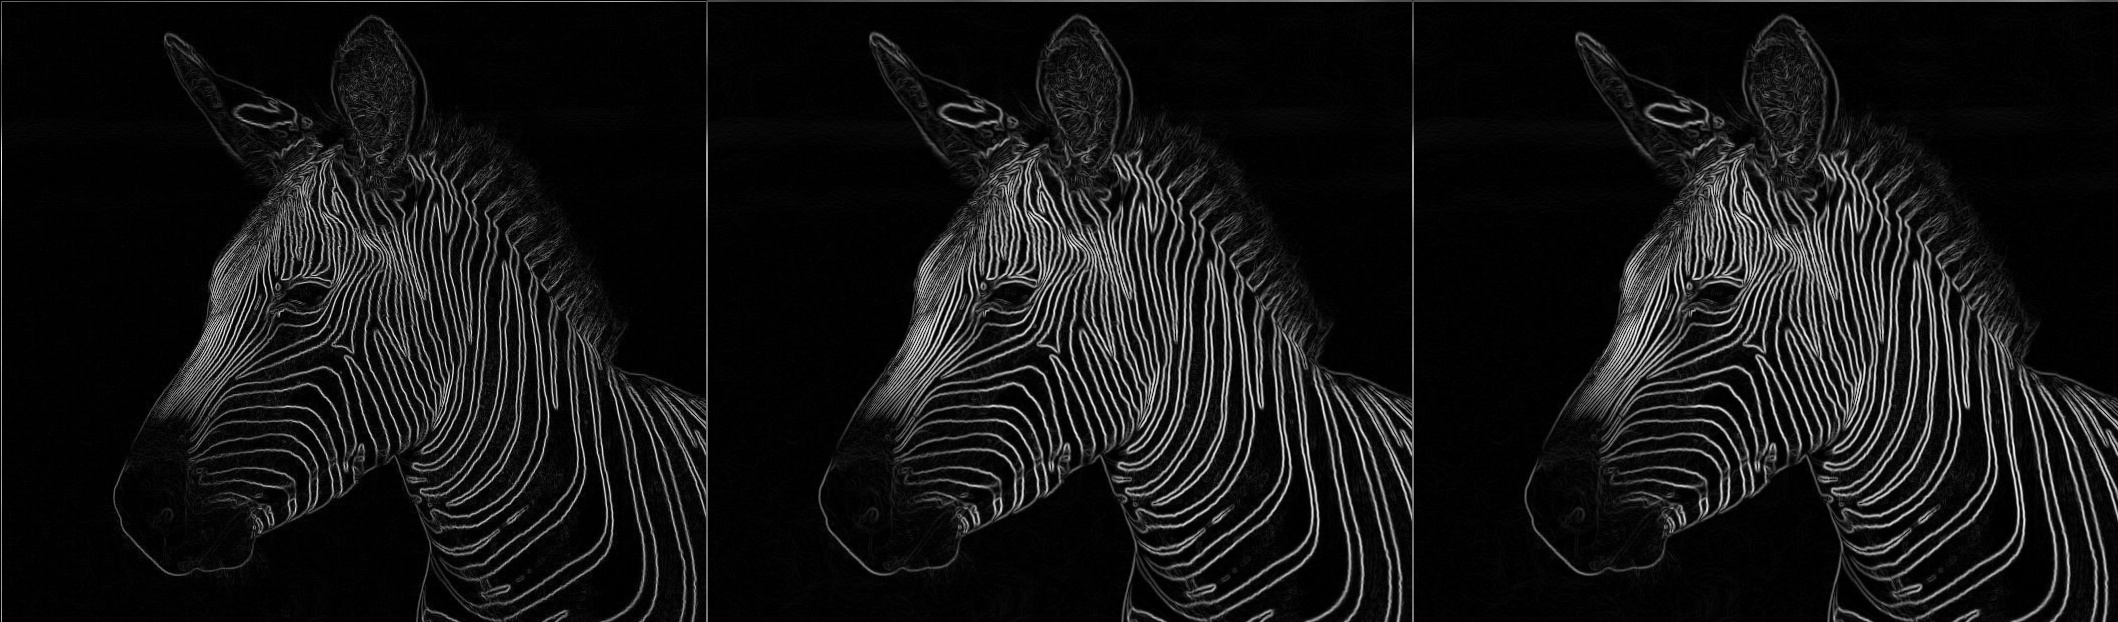
\includegraphics[scale=0.2]{all_sravnenie_2.jpg}
		\caption{Сравнение выделения границ операторами Робертса, Собеля и Превитта на естественном изображении} 
		\label{pic:hist_orig} % название для ссылок внутри кода
	\end{center}
\end{figure}
\begin{figure}[H]
	\begin{center}
		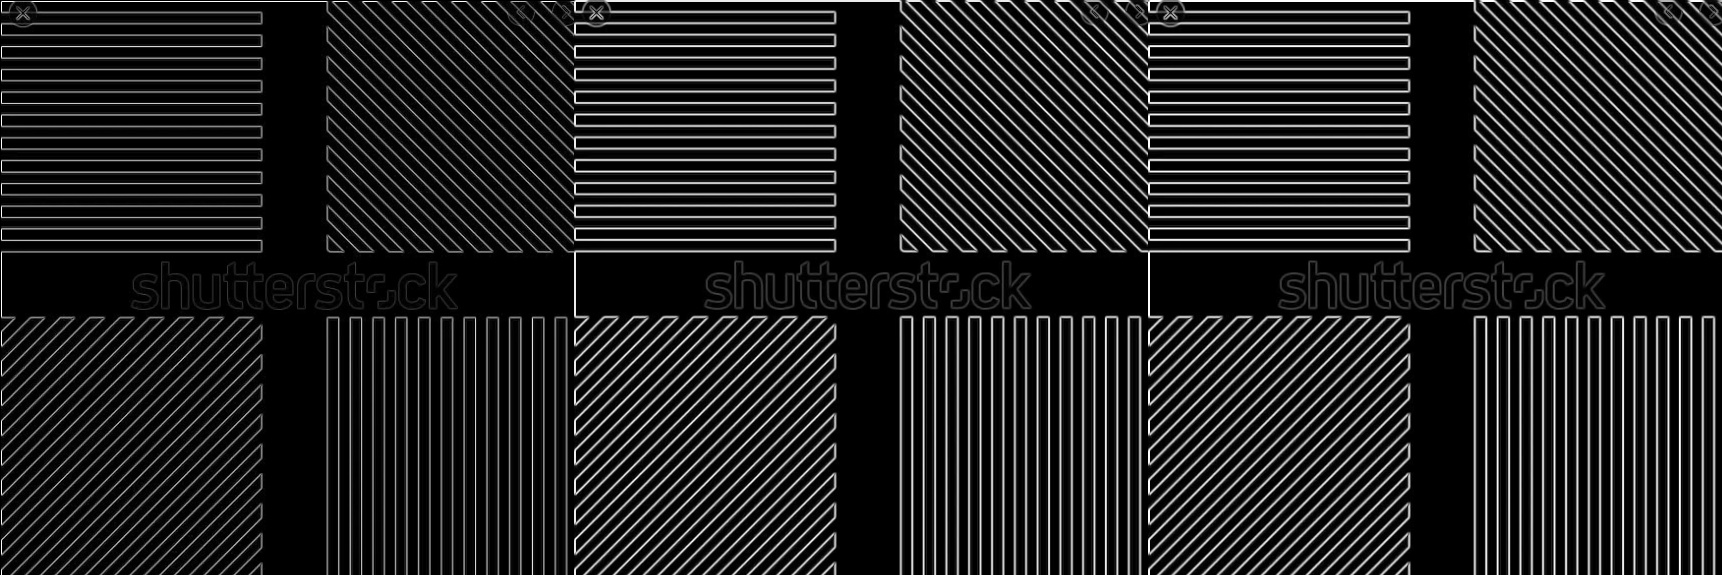
\includegraphics[scale=0.25]{all_sravnenie_1.jpg}
		\caption{Сравнение выделения границ операторами Робертса, Собеля и Превитта на искусственном изображении} 
		\label{pic:hist_orig} % название для ссылок внутри кода
	\end{center}
\end{figure}


\section{Выводы}
Оператор Робертса работает не так качественно как операторы Собеля и Превитта. Оператор Собеля довольно похож на оператор Превитта, а видоизменение заключается в использовании весового коэффициента 2 для средних элементов. Это увеличенное значение используется для уменьшения эффекта сглаживания за счет придания большего веса средним точкам. Этот эффект виден только при большом увеличении изображения
\end{document}
